% Created 2022-11-08 mar 09:49
% Intended LaTeX compiler: pdflatex
\documentclass[presentation]{beamer}
\usepackage[utf8]{inputenc}
\usepackage[T1]{fontenc}
\usepackage{graphicx}
\usepackage{longtable}
\usepackage{wrapfig}
\usepackage{rotating}
\usepackage[normalem]{ulem}
\usepackage{amsmath}
\usepackage{amssymb}
\usepackage{capt-of}
\usepackage{hyperref}
\usepackage{minted}
\usepackage[, french]{babel}
\usepackage{svg}
\usetheme{metropolis}
\usecolortheme{}
\usefonttheme{}
\useinnertheme{}
\useoutertheme{}
\author{Guy Bégin}
\date{\today}
\title{Circuits logiques combinatoires et séquentiels}

\hypersetup{
 pdfauthor={Guy Bégin},
 pdftitle={Circuits logiques combinatoires et séquentiels},
 pdfkeywords={},
 pdfsubject={},
 pdfcreator={Emacs 28.1 (Org mode 9.5.2)}, 
 pdflang={French}}
\begin{document}

\maketitle

\section{Circuits combinatoires typiques}
\label{sec:org6a74347}

\begin{frame}[label={sec:org2759d9b}]{Objectifs}
\begin{itemize}
\item Pouvoir analyser un circuit combinatoire à partir de son schéma
\item Pouvoir concevoir un circuit combinatoire à partir d'une spécification
\item Connaître différentes approches de réalisation
\item Être familier avec les principaux circuits combinatoires courants et
leurs fonctions: additionneur, décodeur, multiplexeur, encodeur,
comparateur
\item Comprendre le fonctionnement d'une chaîne d'addition binaire et les
mécanismes de propagation et d'anticipation de retenue
\end{itemize}
\end{frame}

\begin{frame}[label={sec:orgdd130a5}]{Circuit combinatoire}
\begin{itemize}
\item Un circuit logique combinatoire est une combinaison de portes logiques dont la sortie à un instant donné ne dépend que des valeurs des entrées à cet instant.
\end{itemize}
\end{frame}

\begin{frame}[label={sec:orgaa64f16}]{Circuit combinatoire \ldots{} 2}
\begin{itemize}
\item Un circuit combinatoire à \(n\) entrées et \(m\) sorties peut être représenté par un schéma-bloc, dans lequel on place généralement les entrées à gauche et les sorties à droite.
\end{itemize}

\begin{figure}[htbp]
\centering
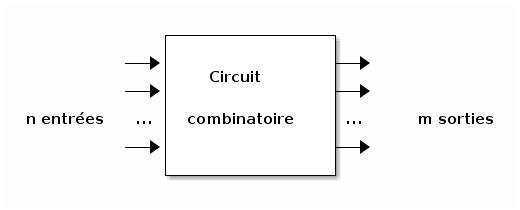
\includegraphics[width=.9\linewidth]{../../Sources_images_logiques/images/circuit_comb.png}
\caption{\label{fig:org75c055c}Circuit combinatoire}
\end{figure}
\end{frame}

\begin{frame}[label={sec:org7a71ccd}]{Circuit combinatoire}
\begin{itemize}
\item Avec \(n\) entrées, il est possible de créer \(2^n\) combinaisons différentes des entrées binaires.

\item Pour chaque combinaison, le circuit peut donner une sortie 0 ou 1.

\item On peut donc préciser la fonction réalisée par le circuit par un tableau de vérité comportant \(2^n\) lignes.

\item Comme nous avons \(m\) sorties différentes, il y aura \(m\) colonnes dans le tableau de vérité pour les fonctions de sortie.

\item Traditionnellement, on présente les entrées en ordre croissant de combinaison binaires.
\end{itemize}
\end{frame}

\begin{frame}[label={sec:orge657b28}]{Analyse d'un circuit logique combinatoire}
\begin{itemize}
\item Si on est placé devant le schéma d'un circuit logique dont on ne connaît pas la fonction, on doit en faire l'analyse.

\item La première étape consiste à vérifier qu'il s'agit bien d'un circuit combinatoire.

\item Si le schéma ne comporte pas de cellules de mémoire ou de boucles de rétroaction, on peut conclure que le circuit est combinatoire.

\item Une boucle de rétroaction consiste en un chemin dans le circuit dans lequel une valeur d'entrée d'une porte provient, directement ou indirectement (par l'intermédiaire d'autres portes), de la sortie de la même porte.

\item La présence de rétroaction est une caractéristique des circuits logiques séquentiels, que nous étudierons plus loin.
\end{itemize}
\end{frame}


\begin{frame}[label={sec:orgb7aa8f4}]{Analyse d'un circuit logique combinatoire \ldots{} 2}
\begin{itemize}
\item Pour interpréter le comportement du circuit, nous devons déterminer les expressions logiques qu'il met en oeuvre ou établir son tableau de vérité.
\end{itemize}


Pour déterminer l'expression logique, on procède ainsi:
\begin{enumerate}
\item Étiqueter toutes les sorties des portes qui sont alimentées par les
variables d'entrée du système. Les noms de variables seront
arbitraire, mais devraient être choisis de façon à faciliter
l'interprétation par la suite. Déterminer les fonctions logiques
pour ces variables.
\item Étiqueter les sorties des portes qui sont alimentées par les
variables d'entrée et par les sorties étiquetées à l'étape
précédente. Déterminer les fonctions logiques pour ces nouvelles
variables.
\end{enumerate}
\end{frame}

\begin{frame}[label={sec:orgfa6ff7b}]{Analyse d'un circuit logique combinatoire \ldots{} 3}
\begin{enumerate}
\setcounter{enumi}{2}
\item Répéter l'étape 2 jusqu'à arriver aux variables de sortie du système.
\item En substituant les expressions logiques des fonctions identifiées,
déterminer l'expression logique pour les sorties du système en
fonction des entrées du système.
\end{enumerate}
\end{frame}

\begin{frame}[label={sec:orge16230e}]{Exemple d'analyse d'un circuit logique combinatoire}
Considérons le circuit combinatoire à analyser illustré à la figure
suivante.

\begin{figure}[htbp]
\centering
\includesvg[scale=0.75]{../../Sources_images_logiques/images/circuit_logique_inconnu}
\caption{\label{fig:org46d24a0}Circuit combinatoire à analyser}
\end{figure}
\end{frame}

\begin{frame}[label={sec:orgcb3e790}]{Exemple d'analyse d'un circuit logique combinatoire \ldots{} 2}
\begin{enumerate}
\item Il n'est pas la peine d'étiqueter la sortie de la porte
inverseur. Comme variables intermédiaire, nous considérons \(I_1\)
en sortie de la porte ET à trois entrées et \(I_2\) en sortie de la
porte NOR. On trouve que \(I_1 = A^\prime \cdot B \cdot C\) et que
\(I_2 = (A + D)^\prime = A^\prime \cdot D^\prime\).

\item On aura donc \(F_1 = I_1 \cdot I_2\).

\item En substituant, \(F_1 = ( A^\prime \cdot B \cdot C ) \cdot (
   A^\prime \cdot D^\prime) = A^\prime \cdot B \cdot C \cdot
   D^\prime\).

\item En simplifiant, on obtient finalement \(F_1 = A^\prime \cdot B
   \cdot C \cdot D^\prime\).
\end{enumerate}
\end{frame}

\begin{frame}[label={sec:org0cb1112}]{Exemple d'analyse d'un circuit logique combinatoire \ldots{} 3}
\begin{table}[h] \scriptsize
\caption{\label{tab:orge8d8e42}Tableaux de vérité des fonctions intermédiaires et de la sortie}
\centering
\begin{tabular}{rrrrlrrr}
\(A\) & \(C\) & \(B\) & \(D\) &  & \(I_1\) & \(I_2\) & \(F_1\)\\
\hline
0 & 0 & 0 & 0 &  & 0 & 0 & 0\\
0 & 0 & 0 & 1 &  & 0 & 0 & 0\\
0 & 1 & 0 & 0 &  & 0 & 1 & 0\\
0 & 1 & 0 & 1 &  & 0 & 0 & 0\\
0 & 0 & 1 & 0 &  & 0 & 1 & 0\\
0 & 0 & 1 & 1 &  & 0 & 0 & 0\\
0 & 1 & 1 & 0 &  & 1 & 1 & 1\\
0 & 1 & 1 & 1 &  & 1 & 0 & 0\\
1 & 0 & 0 & 0 &  & 0 & 0 & 0\\
1 & 0 & 0 & 1 &  & 0 & 0 & 0\\
1 & 1 & 0 & 0 &  & 0 & 0 & 0\\
1 & 1 & 0 & 1 &  & 0 & 0 & 0\\
1 & 0 & 1 & 0 &  & 0 & 0 & 0\\
1 & 0 & 1 & 1 &  & 0 & 0 & 0\\
1 & 1 & 1 & 0 &  & 0 & 0 & 0\\
1 & 1 & 1 & 1 &  & 0 & 0 & 0\\
\end{tabular}
\end{table}
\end{frame}


\begin{frame}[label={sec:org87d3225}]{Conception d'un circuit combinatoire}
\begin{itemize}
\item Concevoir un circuit logique commence avec la formulation de la ou des fonctions du système et se termine avec une implémentation en portes logiques des fonctions logiques correspondantes.
\end{itemize}

Voici les étapes à suivre.

\begin{enumerate}
\item À partir de l'expression du besoin ou des spécifications du
système, déterminer combien d'entrées et de sorties sont
requises, et leur assigner des noms de variables. Le choix des noms
devrait faciliter leur interprétation en lien avec leur fonction.

\item Formuler le tableau de vérité qui décrit les valeurs logiques que
doivent assumer les sorties en fonction des différentes
combinaisons d'entrées.
\end{enumerate}
\end{frame}

\begin{frame}[label={sec:org758ecc4}]{Conception d'un circuit combinatoire \ldots{} 2}
\begin{enumerate}
\setcounter{enumi}{2}
\item Simplifier les expressions logiques pour les différentes fonctions,
en tenant éventuellement compte des partages possibles d'éléments
intermédiaires.

\item Tracer le circuit logique résultant, et le valider (à la main ou
mieux, par simulation).
\end{enumerate}
\end{frame}

\begin{frame}[label={sec:org716820c}]{Conception d'un circuit combinatoire \ldots{} 3}
\begin{itemize}
\item L'étape 2 est cruciale, car ce qui sera implémenté (s'il n'y a pas d'erreurs) est exactement ce que le tableau de vérité spécifie.

\item On doit donc s'assurer que le tableau est correctement rempli et représente véritablement les besoins identifiés.

\item Si des hypothèses ou des choix doivent être faits, notamment dans le cas où l'expression informelle des besoins est incomplète ou ambiguë, ces choix doivent être clairement identifiés et documentés, permettant le cas échéant de les modifier lorsque le système est mis à l'épreuve en fonctionnement.
\end{itemize}
\end{frame}

\begin{frame}[label={sec:org00385db}]{Conception d'un circuit combinatoire \ldots{} 4}
N'importe quelle méthode de simplification peut être utilisée pour l'étape 3, mais il faut aussi prendre en compte 
\begin{itemize}
\item le type de portes disponibles pour l'implémentation,
\item les délais de propagations à travers les portes,
\item le nombre d'interconnexions entre sorties et entrées de portes,
\item et tout autre facteur pratique susceptible d'orienter les décisions finales.
\end{itemize}
\end{frame}

\begin{frame}[label={sec:org5fbec70}]{Alternatives d'implémentation}
\begin{itemize}
\item Considérons la fonction logique \(Y\) correspondant au diag-K de la figure suivante.
\end{itemize}

\begin{figure}[htbp]
\centering
\includesvg[scale=0.75]{../../Sources_images_logiques/images/kmap3altern}
\caption{\label{fig:orgde6aa46}Diag-K d'une fonction combinatoire \(Y\) à réaliser}
\end{figure} 
\end{frame}

\begin{frame}[label={sec:org865a669}]{Implémentations via la fonction directe, en \emph{somme de produits}}
\begin{itemize}
\item En \emph{somme de produits}, on a \(Y = bc + a^\prime b + a b^\prime c^\prime\) pour la fonction et \(Y^\prime = a^\prime b^\prime + b^\prime c + a b c^\prime\) pour son complément.

\item Les implémentations possibles pour la fonction directe sont illustrées ci-dessous.
\end{itemize}
\end{frame}

\begin{frame}[label={sec:org93672ac}]{Implémentations via la fonction directe, en \emph{somme de produits}}
\begin{figure}[htbp]
\centering
\includesvg[scale=0.75]{../../Sources_images_logiques/images/circ_altern_1}
\caption{\label{fig:orgd7850b0}Implémentation de \(Y\) en \emph{somme de produits}}
\end{figure} 
\end{frame}

\begin{frame}[label={sec:orgdec0bcb}]{Implémentations via la fonction directe, en \emph{somme de produits} \ldots{} 2}
\begin{figure}[htbp]
\centering
\includesvg[scale=0.75]{../../Sources_images_logiques/images/circ_altern_2}
\caption{\label{fig:orgf6829fa}Implémentation (en NAND) de \(Y\) en \emph{somme de produits}}
\end{figure} 
\end{frame}


\begin{frame}[label={sec:org815df0a}]{Implémentation en \emph{produit de sommes}}
\begin{itemize}
\item En \emph{produit de sommes}, on a \(Y =(a + b ) (b + c^\prime ) (a^\prime + ba^\prime + c)\) pour la fonction et \(Y^\prime = (b^\prime +c^\prime )(a+b^\prime )(a^\prime +b+c)\) pour son complément.

\item Les implémentations possibles pour la fonction directe sont illustrées ci-dessous.
\end{itemize}
\end{frame}

\begin{frame}[label={sec:org709e1c0}]{Implémentation en \emph{produit de sommes} \ldots{} 2}
\begin{figure}[htbp]
\centering
\includesvg[scale=0.75]{../../Sources_images_logiques/images/circ_altern_ps1}
\caption{\label{fig:org1c8d7ca}Implémentation de \(Y\) en \emph{produit de sommes}}
\end{figure} 
\end{frame}

\begin{frame}[label={sec:org183d89b}]{Implémentation en \emph{produit de sommes} \ldots{} 3}
\begin{figure}[htbp]
\centering
\includesvg[scale=0.75]{../../Sources_images_logiques/images/circ_altern_ps2}
\caption{\label{fig:org80baa71}Implémentation (en NOR) de \(Y\) en \emph{produit de sommes}}
\end{figure} 
\end{frame}


\begin{frame}[label={sec:org6b92819}]{Implémentations via la fonction complémentaire}
\begin{itemize}
\item On peut aussi implémenter la fonction à partir de la fonction complémentaire \(Y^\prime\), en se basant sur le complément \(Y^\prime = (b^\prime +c^\prime )(a+b^\prime )(a^\prime +b+c)\) et en inversant la sortie.

\item Voici les implémentations que l'on obtient alors.
\end{itemize}
\end{frame}

\begin{frame}[label={sec:org5a39c8b}]{Implémentation via la fonction complémentaire, en \emph{somme de produits}}
\begin{itemize}
\item En \emph{somme de produits}, on a utilisé une porte NOR en sortie pour obtenir finalement \(Y\).
\end{itemize}

\begin{figure}[htbp]
\centering
\includesvg[scale=0.75]{../../Sources_images_logiques/images/circ_altern_comp_sp1}
\caption{\label{fig:org7b5e1d3}Implémentation via \(Y^\prime\) en \emph{somme de produits}}
\end{figure} 
\end{frame}

\begin{frame}[label={sec:org0819b32}]{Implémentation via la fonction complémentaire, en \emph{somme de produits} \ldots{} 2}
\begin{itemize}
\item Une autre forme fait appel à des portes NAND au premier niveau.
\end{itemize}

\begin{figure}[htbp]
\centering
\includesvg[scale=0.75]{../../Sources_images_logiques/images/circ_altern_comp_sp2}
\caption{\label{fig:org822cca5}Implémentation via \(Y^\prime\) en \emph{somme de produits}}
\end{figure} 
\end{frame}

\begin{frame}[label={sec:org3dba2d9}]{Implémentation via la fonction complémentaire, en \emph{produit de sommes}}
\begin{itemize}
\item En \emph{produit de sommes}, en se basant sur le complément \(Y^\prime = (b^\prime +c^\prime )(a+b^\prime )(a^\prime +b+c)\).

\item On a encore ici deux variantes selon le type de portes utilisées.
\end{itemize}

\begin{figure}[htbp]
\centering
\includesvg[scale=0.75]{../../Sources_images_logiques/images/circ_altern_comp_ps1}
\caption{\label{fig:org74a3a00}Implémentation via \(Y^\prime\) en \emph{produit de sommes}}
\end{figure} 
\end{frame}

\begin{frame}[label={sec:org000c2d3}]{Implémentation via la fonction complémentaire, en \emph{produit de sommes} \ldots{} 2}
\begin{figure}[htbp]
\centering
\includesvg[scale=0.75]{../../Sources_images_logiques/images/circ_altern_comp_ps2}
\caption{\label{fig:orgee3960a}Implémentation via \(Y^\prime\) en \emph{produit de sommes}}
\end{figure} 
\end{frame}

\begin{frame}[label={sec:org9619208}]{Circuits logiques combinatoires classiques}
\begin{itemize}
\item Nous allons maintenant nous intéresser à un certain nombre de fonctions typiques que l'on rencontre fréquemment en circuits logiques.

\item Ce sera aussi l'occasion de mettre en pratique les approches de conception que nous avons vues.
\end{itemize}
\end{frame}


\begin{frame}[label={sec:org4a7c552}]{Additionneur binaire}
\begin{itemize}
\item Une des opérations binaires les plus utilisées est l'addition (et la soustraction).

\item Nous avons présenté précédemment le tableau de vérité pour un additionneur binaire dont les entrées sont \(a_{i}\) et \(b_{i}\), les bits des nombres à additionner, et aussi \(r_{i-1}\), la retenue provenant de la position \(i-1\).

\item En sortie, on aura la somme \(S_{i}\) et la retenue \(R_{i}\).

\item Notez que pour bien distinguer la retenue d'entrée de la retenue de sortie, nous utilisons un symbole minuscule, \(r_{i-1}\), pour l'entrée et un symbole majuscule, \(R_{i}\), pour la sortie.
\end{itemize}
\end{frame}

\begin{frame}[label={sec:orgd69c7ed}]{Additionneur binaire \ldots{} 2}
\begin{figure}[htbp]
\centering
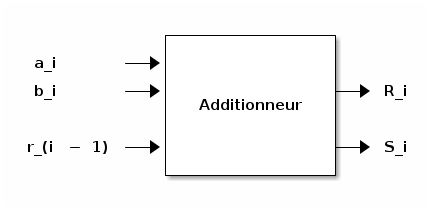
\includegraphics[scale=0.75]{../../Sources_images_logiques/images/additionneur.png}
\caption{\label{fig:orgc72f15a}Schéma-bloc d'un additionneur complet}
\end{figure}
\end{frame}

\begin{frame}[label={sec:org9abc3ca}]{Additionneur binaire \ldots{} 3}
\begin{table}[htbp]
\caption{\label{tab:org9afe4fc}Tableau de vérité pour l'additionneur binaire}
\centering
\begin{tabular}{rrrlrr}
\(a_{i}\) & \(b_{i}\) & \(r_{i-1}\) &  & \(R_{i}\) & \(S_{i}\)\\
\hline
0 & 0 & 0 &  & 0 & 0\\
0 & 0 & 1 &  & 0 & 1\\
0 & 1 & 0 &  & 0 & 1\\
0 & 1 & 1 &  & 1 & 0\\
1 & 0 & 0 &  & 0 & 1\\
1 & 0 & 1 &  & 1 & 0\\
1 & 1 & 0 &  & 1 & 0\\
1 & 1 & 1 &  & 1 & 1\\
\end{tabular}
\end{table}
\end{frame}


\begin{frame}[label={sec:org52ba8bd}]{Demi-additionneur}
\begin{itemize}
\item Un circuit logique qui effectue l'addition de deux bits est appelé un demi-additionneur.

\item Mais ce qu'il nous faut vraiment, c'est un \alert{additionneur complet}, c'est-à-dire, un circuit de trois entrées qui fait l’addition de trois bits, puisqu'il faudra pouvoir tenir compte de la retenue du niveau précédent pour effectuer l'addition sur un niveau.

\item Il est possible d'implémenter l'additionneur complet avec deux demi-additionneurs.
\end{itemize}
\end{frame}

\begin{frame}[label={sec:org5263dfa}]{Demi-additionneur \ldots{} 2}
\begin{table}[htbp]
\caption{\label{tab:orgf332910}Tableau de vérité pour un demi-additionneur}
\centering
\begin{tabular}{rrlrr}
\(a_{i}\) & \(b_{i}\) &  & \(R_{i}\) & \(S_{i}\)\\
\hline
0 & 0 &  & 0 & 0\\
0 & 1 &  & 0 & 1\\
1 & 0 &  & 0 & 1\\
1 & 1 &  & 1 & 0\\
\end{tabular}
\end{table}
\end{frame}

\begin{frame}[label={sec:org9343fc0}]{Demi-additionneur \ldots{} 3}
\begin{itemize}
\item À partir du tableau de vérité, on peut trouver que pour un demi-additionneur, \(S_{i} = a_i b_i^\prime + a_i^\prime b_i = a_i \operatorname{Xor} b_i\) et \(R_{i} = a_i b_i\).
\end{itemize}

\begin{figure}[htbp]
\centering
\includesvg[scale=0.75]{../../Sources_images_logiques/images/demi_add2}
\caption{\label{fig:orgc9424e9}Circuit demi-additionneur (en S de P)}
\end{figure}
\end{frame}

\begin{frame}[label={sec:org5f43190}]{Demi-additionneur \ldots{} 4}
\begin{figure}[htbp]
\centering
\includesvg[scale=0.75]{../../Sources_images_logiques/images/demi_add}
\caption{\label{fig:org058dbb3}Circuit demi-additionneur avec porte XOR}
\end{figure}
\end{frame}

\begin{frame}[label={sec:org5dbc6d2}]{Additionneur complet}
\begin{itemize}
\item Une addition binaire complète de deux arguments constitués de \(n\) bits procède du bit le moins significatif vers le bits le plus significatif, en additionnant à chaque étape trois bits: \(a_{i}\), \(b_{i}\) et \(r_{i-1}\) et en produisant une somme \(S_{i}\) et une retenue \(R_{i}\).
\end{itemize}


\begin{figure}[htbp]
\centering
\includesvg[scale=0.75]{../../Sources_images_logiques/images/kmapSi_fulladder}
\caption{\label{fig:org0b8c5d2}Diag-K pour \(S_i\), additionneur complet}
\end{figure}
\end{frame}

\begin{frame}[label={sec:orgd36481e}]{Additionneur complet \ldots{} 2}
\begin{figure}[htbp]
\centering
\includesvg[scale=0.75]{../../Sources_images_logiques/images/kmap3fulladderR}
\caption{\label{fig:org86d1473}Diag-K pour \(R_i\), additionneur complet}
\end{figure}
\end{frame}

\begin{frame}[label={sec:orgc753bad}]{Additionneur complet \ldots{} 3}
Les expressions simplifiées sont 

$$ S_{i} = a_i^\prime b_i^\prime r_{i-1} + a_i^\prime b_i
r_{i-1}^\prime + a_i b_i^\prime r_{i-1}^\prime + a_i b_i r_{i-1} $$

$$ R_{i} = a_i b_i + a_i r_{i-1} + b_i r_{i-1} $$
\end{frame}

\begin{frame}[label={sec:org28d5e00}]{Additionneur complet \ldots{} 4}
\begin{figure}[htbp]
\centering
\includesvg[scale=0.75]{../../Sources_images_logiques/images/fulladderS}
\caption{\label{fig:org14ccb9c}Circuit additionneur complet pour \(S_i\)}
\end{figure}
\end{frame}

\begin{frame}[label={sec:org3132ccd}]{Additionneur complet \ldots{} 5}
\begin{figure}[htbp]
\centering
\includesvg[scale=0.75]{../../Sources_images_logiques/images/fulladderR}
\caption{\label{fig:orgea817c0}Circuit additionneur complet pour \(R_i\)}
\end{figure}
\end{frame}

\begin{frame}[label={sec:orgecfe44a}]{Additionneur complet \ldots{} 6}
Comme on le disait précédemment, il est possible de combiner deux
demi-additionneurs pour réaliser un additionneur complet, comme on
peut le voir ici.


\begin{figure}[htbp]
\centering
\includesvg[scale=0.75]{../../Sources_images_logiques/images/fulladderxor}
\caption{\label{fig:orgad9ef67}Circuit additionneur complet comportant deux demi-additionneurs et une porte OU}
\end{figure}
\end{frame}

\begin{frame}[label={sec:orgd3c172c}]{Additionneur binaire pour \(n\) bits}
\begin{itemize}
\item Un additionneur binaire est un circuit logique qui permet d'évaluer la somme arithmétique de deux nombres binaire de \(n\) bits.

\item Il peut être conçu en combinant des additionneurs complets en cascade, en reliant la retenue de sortie provenant de la position 0 (la moins significative) à l'entrée de retenue de la position 1, \ldots{}, la retenue de sortie provenant de la position \(i-1\) à l'entrée de retenue de la position \(i\), etc. (figure \ref{fig:org14822a5}).

\item Pour en faire un circuit général pouvant également se combiner en chaîne, on prévoit une entrée pour une retenue au niveau 0, \(r_0\) et une sortie pour une retenue du dernier niveau \(n-1\), \(R_{n-1}\).

\item On doit donc, pour le chaînage, acheminer la sortie retenue du niveau courant à l'entrée de retenue du niveau suivant.
\end{itemize}
\end{frame}

\begin{frame}[label={sec:orgbd5c0ad}]{Chaîne d'addition}
\begin{figure}[htbp]
\centering
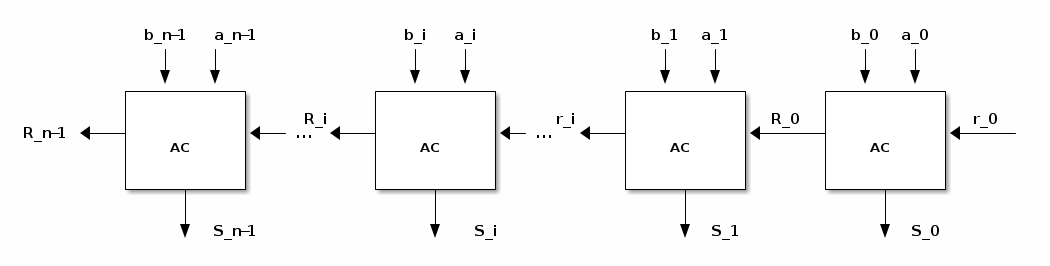
\includegraphics[width=.9\linewidth]{../../Sources_images_logiques/images/additionneur_cascade.png}
\caption{\label{fig:org14822a5}Chaîne d'addition}
\end{figure}
\end{frame}

\begin{frame}[label={sec:orgc56a162}]{Chaîne d'addition \ldots{} 2}
\begin{itemize}
\item Cette réalisation en forme de chaîne, en réutilisant de façon systématique un bloc élémentaire, est avantageuse d'un point de vue complexité et flexibilité.

\item Imaginons par exemple le défi de concevoir un additionneur binaire pour des nombres de quatre bits par la méthode classique.

\item Comme il faudrait considérer 9 entrées, le tableau de vérité comporterait \(2^9= 512\) lignes!
\end{itemize}
\end{frame}

\begin{frame}[label={sec:orgf167806}]{Propagation de retenue}
\begin{itemize}
\item L'approche en cascade ne comporte pas que des avantages.

\item Lorsqu'on effectue l'addition de deux nombres, les bits d'entrée des deux arguments et la retenue d'entrée sont présentés en même temps à l'additionneur.

\item Comme dans tout circuit combinatoire, il faut un certain délai avant que les sorties n'atteignent leur niveau de sortie final.

\item Ce délai de propagation dépend de la profondeur du circuit, en nombre de portes élémentaires à franchir de l'entrée vers la sortie.

\item Et c'est évidemment le chemin le plus long qui détermine le délai de propagation global.
\end{itemize}
\end{frame}

\begin{frame}[label={sec:orgecbdfd6}]{Propagation de retenue \ldots{} 2}
\begin{itemize}
\item Dans le cas de l'additionneur, le chemin de propagation le plus long est celui qui mène à la dernière retenue finale \(R_{n-1}\).

\item En effet, pour pouvoir calculer \(R_{n-1}\), bien que les valeurs de \(a_{n-1}\) et \(b_{n-1}\) soient déjà disponibles, il faut attendre que la valeur de \(r_{n-1} = R_{n-2}\) soit stabilisée avant que le calcul puisse s'effectuer avec les bonnes valeurs.

\item Il en est de même avec la bloc précédent, et ainsi, en remontant la chaîne vers \(r_0\), on trouve le chemin de propagation de retenue comme chemin le plus long.
\end{itemize}
\end{frame}

\begin{frame}[label={sec:orgd2dedb3}]{Propagation de retenue \ldots{} 3}
\begin{itemize}
\item Pour déterminer le nombre de portes à franchir pour le chemin de propagation de retenue, nous avons ajouté deux sorties intermédiaires à notre circuit d'additionneur complet, \(P_i\) et \(G_i\), permettant de récrire la sortie comme \(S_i = P_i \operatorname{Xor} r_i\) et la retenue de sortie comme \(R_i = P_i r_i + G_i\).

\item Les signaux \(P_i\) et \(G_i\) ne dépendent que des entrées et sont donc disponibles après le délai des portes ET et XOR.

\item Le chemin de \(r_i\) à \(R_i\) passe par une porte ET et une porte OU.

\item Pour un additionneur de \(n\) bits comprenant \(n\) additionneurs complets, on aura une profondeur de retenue totale de \(2n\) portes.
\end{itemize}
\end{frame}

\begin{frame}[label={sec:orga175843}]{Propagation de retenue \ldots{} 4}
\begin{figure}[htbp]
\centering
\includesvg[width=.9\linewidth]{../../Sources_images_logiques/images/fulladderxorPG}
\caption{\label{fig:org9220dbf}Circuit additionneur complet montrant les signaux intermédiaires \(P_i\) et \(G_i\)}
\end{figure}
\end{frame}

\begin{frame}[label={sec:orgf1beb96}]{Anticipation de retenue}
\begin{itemize}
\item Les valeurs calculées par le circuit complet en chaîne ne seront valides et ne devront être prises en compte que lorsque le délai maximal se sera écoulé.

\item Entre temps, les valeurs binaires présentes aux différentes sorties assumeront typiquement des valeurs changeantes jusqu'à stabilisation finale.

\item Le délai de propagation de retenue est un facteur qui limite la vitesse à laquelle on pourra calculer la somme de deux nombres.

\item Et comme l'addition est une opération courante, souvent utilisée, parfois à répétition, pour réaliser d'autres opérations arithmétiques, cette limitation est problématique.
\end{itemize}
\end{frame}

\begin{frame}[label={sec:org4311d76}]{Anticipation de retenue \ldots{} 2}
\begin{itemize}
\item Il serait en théorie possible de ramener à un minimum le délai de calcul de la retenue finale en réalisant cette fonction en deux niveaux, par exemple avec un \emph{produit de sommes}.

\item Cette option n'est pas réaliste, car le nombre d'entrées à considérer en parallèle est prohibitif.

\item Comme solutions de compromis intermédiaires, un certain nombre de mécanismes ont été élaborés, dont l'approche par anticipation de retenue, que nous allons explorer ici.
\end{itemize}
\end{frame}

\begin{frame}[label={sec:org3594a35}]{Anticipation de retenue \ldots{} 3}
\begin{itemize}
\item On fait appel aux deux signaux \(P_i = a_i \operatorname{Xor} b_i\) et \(G_i = a_i b_i\), qui donnent respectivement pour la sortie et la retenue de sortie
\end{itemize}

$$ S_i = P_i \operatorname{Xor} r_{i-1} $$
$$ R_i = P_i r_{i-1} + G_i $$

\begin{itemize}
\item \(G_i\) est le signal qui indique la \alert{génération} de retenue, produisant une retenue lorsque \(a_i\) et \(b_i\) sont tous deux à 1, sans égard à la valeur de la retenue d'entrée \(r_{i-1}\).

\item Le signal \(P_i\) est l'indicateur de \alert{propagation} de retenue, parce qu'il détermine si la retenue du niveau précédent \(r_{i-1}\) sera propagée à \(R_i\).
\end{itemize}
\end{frame}

\begin{frame}[label={sec:org56a64f7}]{Anticipation de retenue \ldots{} 4}
En partant du niveau 0, voici les expressions pour les différentes retenues:

$$ R_0 = r_0 = \operatorname{in}$$
$$ R_1 = G_0 + P_0 R_0 $$
$$ R_2 = G_1 + P_1 R_1 = G_1 + P_1 (G_0 + P_0 R_0) = G_1 + P_1 G_0 + P_1 P_0 R_0 $$
$$ R_3 = G_2 + P_2 R_2 = G_2 + P_2 G_1 + P_2 P_1 G_0 + P_2 P_1 P_0 R_0 $$
etc.
\end{frame}

\begin{frame}[label={sec:org42a7ccc}]{Anticipation de retenue \ldots{} 5}
\begin{itemize}
\item Les expressions pour les retenues successives sont en forme \emph{somme de produits}, ce qui mène à une implémentation à deux niveaux pour calculer les retenues rapidement.

\item Contrairement à l'approche de propagation de retenue, toutes les retenues sont obtenues après un même délai équivalent à une profondeur de deux portes.

\item En calculant d'abord les différentes valeurs de \(P_i\) et \(G_i\) pour chaque niveau et en utilisant ces résultats intermédiaires pour, d'une part alimenter le circuit d'anticipateur de retenue et d'autre part, effectuer \(S_i = P_i \operatorname{Xor} r_i\), on obtient un additionneur parallèle plus rapide que la configuration en cascade.
\end{itemize}
\end{frame}

\begin{frame}[label={sec:orgcf2039d}]{Anticipation de retenue \ldots{} 6}
\begin{figure}[htbp]
\centering
\includesvg[scale=0.55]{../../Sources_images_logiques/images/lookahead1}
\caption{\label{fig:orga67bd5d}Circuit d'anticipateur de retenue pour \(n= 4\)}
\end{figure}
\end{frame}


\begin{frame}[label={sec:org7e1490e}]{Soustraction}
\begin{itemize}
\item Pour effectuer une soustraction \(A - B\), il faut effectuer \(A + (-B)\), c’est-à-dire additionner le complément à deux de \(B\) à \(A\).

\item On détermine le complément à deux en obtenant d'abord le complément à un en complémentant chaque bit, et en additionnant ensuite 1 à cette valeur par le biais de l'entrée de retenue de l'additionneur.
\end{itemize}
\end{frame}

\begin{frame}[label={sec:org7ce38c0}]{Soustraction \ldots{} 2}
\begin{itemize}
\item Il est ainsi possible de concevoir un additionneur/soustracteur commandé par un signal de contrôle \(O\).

\item Si \(O=0\), le circuit calcule \(A + (B)\) et si \(O=1\), le circuit calcule \(A + (-B)\).

\item La complémentation de \(B\) se fait au moyen de portes XOR qui calculent \(O \operatorname{Xor} b_i\) et dont la sortie est acheminée à l'entrée \(B\) de l'additionneur.

\item Lorsque que \(O=1\), leur sortie vaut \(b_i^\prime\).
\end{itemize}
\end{frame}

\begin{frame}[label={sec:org62bea52}]{Soustraction \ldots{} 2}
\begin{figure}[htbp]
\centering
\includesvg[width=.9\linewidth]{../../Sources_images_logiques/images/add_sous}
\caption{\label{fig:org3d25702}Circuit additionneur/ soustracteur 4 bits}
\end{figure}
\end{frame}

\begin{frame}[label={sec:org39de452}]{Débordements}
\begin{itemize}
\item Un additionneur ou un soustracteur sont conçus en fonction d'une taille de nombres \(n\).

\item Lorsque le résultat de l'opération dépasse la limite pouvant être représentée, on doit détecter cette condition et la signaler par un signal binaire.

\item Le cas de l'addition de nombre non signés est le plus simple.

\item Il suffit de surveiller la retenue du niveau le plus significatif.

\item Une retenue de 1 signifie un débordement de l'addition.
\end{itemize}
\end{frame}

\begin{frame}[label={sec:orgbe7436c}]{Débordements: nombre signés}
\begin{itemize}
\item Les calculs avec des nombres signés en complément à deux peuvent aussi occasionner des débordements, mais la détection doit tenir compte des bits qui indiquent le signe des nombres.

\item L'addition de deux nombres de signes différents ne peut pas occasionner de débordement, puisque la valeur absolue du résultat sera nécessairement moindre que celle du plus grand des nombres initiaux.

\item Un débordement ne peut donc se produire que si les deux nombres additionnés sont de même signe, deux positifs ou deux négatifs.
\end{itemize}
\end{frame}

\begin{frame}[label={sec:orge46155b}]{Débordements: illustration}
\begin{itemize}
\item Prenons le cas de nombres représentés sur huit bits en complément à deux.

\item La gamme représentable va de -128 à +127 avec un bit qui représente le signe.

\item Si on additionne (+50)10 = (00110010)2 avec (+100)10 = (01100100)2, on aura un débordement, car \(150 > 127\).

\item On voit dans le tableau suivant les bits qui seront produits par l'addition, avec en évidence les retenues des deux derniers niveaux.

\item Le bit de signe a été séparé des autres.
\end{itemize}
\end{frame}

\begin{frame}[label={sec:org2d65a19}]{Débordements: deux positifs}
\begin{table}[htbp]
\caption{\label{tab:orge8825a0}Addition de (+50)10 + (+100)10 = (00110010)2 + (01100100)2}
\centering
\begin{tabular}{lrrl}
Retenues & 0 & 1 & \\
\hline
 &  & 0 & 011 0010\\
 &  & 0 & 110 0100\\
\hline
 &  & 1 & 001 0110\\
\end{tabular}
\end{table}
\end{frame}

\begin{frame}[label={sec:org232aebb}]{Débordements: deux négatifs}
\begin{itemize}
\item Refaisons le même exercice avec deux nombres négatifs: on additionne (-50)10 = (1100 1110)2 avec (-100)10 = (1001 1100)2, qui créera un débordement aussi.
\end{itemize}

\begin{table}[htbp]
\caption{\label{tab:orgf61a85e}Addition de (-50)10 + (-100)10 = (1100 1110)2 + (1001 1100)2}
\centering
\begin{tabular}{lrrl}
Retenues & 1 & 0 & \\
\hline
 &  & 1 & 100 1110\\
 &  & 1 & 001 1100\\
\hline
 &  & 0 & 110 1010\\
\end{tabular}
\end{table}
\end{frame}

\begin{frame}[label={sec:org988773c}]{Débordements: règle générale}
\begin{itemize}
\item On peut dans les deux cas détecter le débordement en observant que la retenue du dernier niveau et la retenue de l'avant dernier niveau sont différentes.

\item On peut vérifier facilement que les autres cas sans débordement donnent des retenues égales.

\item Donc, si on fait un OU-exclusif entre ces deux retenues, un résultat 1 indiquera un débordement.

\item Ce mécanisme de détection de débordement a été ajouté au circuit additionneur/soustracteur 4 bits dans la figure suivante pour générer le signal \(D\) qui indique un débordement.
\end{itemize}
\end{frame}

\begin{frame}[label={sec:org3f610c2}]{Détection de débordements}
\begin{figure}[htbp]
\centering
\includesvg[width=.9\linewidth]{../../Sources_images_logiques/images/add_sous_deb}
\caption{\label{fig:org2ace8d4}Circuit additionneur/soustracteur 4 bits avec débordement}
\end{figure}
\end{frame}


\begin{frame}[label={sec:org70d71ea}]{Multiplexeur}
\begin{itemize}
\item Un multiplexeur est un circuit combinatoire qui sélectionne le signal qui provient d'une de ses entrées, et fait que sa sortie soit égale à l'entrée sélectionnée.

\item Les signaux de sélection fonctionnent typiquement selon un encodage binaire, ce qui suppose un nombre d'entrées de la forme \(2^n\).

\item On désigne le multiplexeur par le nombre de signaux d'entrées à sélectionner.
\end{itemize}
\end{frame}

\begin{frame}[label={sec:orgc3a0f25}]{Multiplexeur deux-vers-un}
\begin{itemize}
\item Le multiplexeur le plus simple utilise un seul signal de sélection \(S\) qui permet de choisir une de deux entrées \(I_0\) ou \(I_1\) pour agir sur la sortie \(Y\).
\end{itemize}

\begin{figure}[htbp]
\centering
\includesvg[scale=0.75]{../../Sources_images_logiques/images/mux2b}
\caption{\label{fig:orgae36054}Circuit du multiplexeur deux-vers-un}
\end{figure}
\end{frame}

\begin{frame}[label={sec:org4bd10f3}]{Multiplexeur deux-vers-un: symbole}
\begin{figure}[htbp]
\centering
\includesvg[scale=0.75]{../../Sources_images_logiques/images/mux2symb}
\caption{\label{fig:orgb19c73a}Symbole du multiplexeur deux-vers-un}
\end{figure}
\end{frame}

\begin{frame}[label={sec:org2e4bd65}]{Multiplexeur quatre-vers-un}
\begin{itemize}
\item Un multiplexeur quatre-vers-un permet de choisir une de quatre entrées en utilisant deux signaux de sélection.

\item Pour simplifier la représentation symbolique, les deux signaux de sélection sont représentés comme un seul fil, qui correspond en fait à une paire de signaux \(S_0\) et \(S_1\).

\item Pour un multiplexeur à \(2^n\) entrées, on aurait un vecteur de \(n\) signaux de sélection.
\end{itemize}
\end{frame}

\begin{frame}[label={sec:orgdcfd580}]{Multiplexeur quatre-vers-un \ldots{} 2}
\begin{figure}[htbp]
\centering
\includesvg[scale=0.75]{../../Sources_images_logiques/images/mux4}
\caption{\label{fig:org9b9c930}Circuit du multiplexeur quatre-vers-un}
\end{figure}
\end{frame}

\begin{frame}[label={sec:orgc428ddc}]{Multiplexeur quatre-vers-un \ldots{} 3}
\begin{figure}[htbp]
\centering
\includesvg[scale=0.75]{../../Sources_images_logiques/images/mux4symb}
\caption{\label{fig:orgbdc3655}Symbole du multiplexeur quatre-vers-un}
\end{figure}
\end{frame}

\begin{frame}[label={sec:orge729f6b}]{Multiplexeur quatre-vers-un \ldots{} 4}
\begin{table}[htbp]
\caption{\label{tab:org03c76fb}Tableau de vérité du multiplexeur quatre-vers-un}
\centering
\begin{tabular}{rrll}
\(S_1\) & \(S_0\) &  & \(Y\)\\
\hline
0 & 0 &  & \(I_0\)\\
0 & 1 &  & \(I_1\)\\
1 & 0 &  & \(I_2\)\\
1 & 1 &  & \(I_3\)\\
\end{tabular}
\end{table}
\end{frame}



\begin{frame}[label={sec:org06a0c55}]{Décodeur}
\begin{itemize}
\item Un décodeur est un circuit combinatoire qui sert à interpréter des données encodées, le plus souvent en binaire.

\item Il prend un groupe (vecteur) de \(n\) bits en entrée, et active une sortie parmi jusqu'à \(2^n\) sorties différentes.

\item Dans le cas où certaines combinaisons d'entrées ne sont pas utilisées, moins de \(2^n\) sorties peuvent être produites.

\item Dans un décodeur générique, chaque combinaison binaire distincte activera une seule sortie.

\item Il y a une correspondance directe entre chaque sortie possible et un minterm d'entrée.
\end{itemize}
\end{frame}

\begin{frame}[label={sec:org9b87085}]{Décodeur \ldots{} 2}
\begin{figure}[htbp]
\centering
\includesvg[scale=0.55]{../../Sources_images_logiques/images/decod3_8}
\caption{\label{fig:org9275188}Circuit du décodeur trois-vers-huit}
\end{figure}
\end{frame}

\begin{frame}[label={sec:org9d7b39b}]{Décodeur \ldots{} 3}
\begin{table}[htbp]
\caption{\label{tab:orge73f35a}Tableau de vérité du décodeur trois-vers-huit}
\centering
\begin{tabular}{rrrlrrrrrrrr}
\(x\) & \(y\) & \(z\) &  & \(D_0\) & \(D_1\) & \(D_2\) & \(D_3\) & \(D_4\) & \(D_5\) & \(D_6\) & \(D_7\)\\
\hline
0 & 0 & 0 &  & 1 & 0 & 0 & 0 & 0 & 0 & 0 & 0\\
0 & 0 & 1 &  & 0 & 1 & 0 & 0 & 0 & 0 & 0 & 0\\
0 & 1 & 0 &  & 0 & 0 & 1 & 0 & 0 & 0 & 0 & 0\\
0 & 1 & 1 &  & 0 & 0 & 0 & 1 & 0 & 0 & 0 & 0\\
1 & 0 & 0 &  & 0 & 0 & 0 & 0 & 1 & 0 & 0 & 0\\
1 & 0 & 1 &  & 0 & 0 & 0 & 0 & 0 & 1 & 0 & 0\\
1 & 1 & 0 &  & 0 & 0 & 0 & 0 & 0 & 0 & 1 & 0\\
1 & 1 & 1 &  & 0 & 0 & 0 & 0 & 0 & 0 & 0 & 1\\
\end{tabular}
\end{table}
\end{frame}

\begin{frame}[label={sec:org3e5dbed}]{Décodeur avec sortie active basse et signal de contrôle}
\begin{itemize}
\item On peut aussi concevoir des décodeurs basés sur des portes NAND et dont la sortie sélectionnée est active au niveau bas.

\item Une autre fonction utile est un signal de contrôle \(E\) qui n'active une sortie que lorsqu'il est activé.

\item Le décodeur deux-vers-quatre dont le circuit est présenté ci-dessous présente ces deux caractéristiques.

\item Comme on peut voir dans le tableau de vérité, tant que le signal de contrôle est inactif ( \(E = 1\) puisque ce signal est également actif bas), les sorties sont inactives (au niveau 1) quelles que soient les entrées \(x\) et \(y\).

\item Lorsque \(E = 0\), une seule sortie passe à 0, selon le code binaire présent aux entrées \(x\) et \(y\).

\item Notez que tel que conçu et étiqueté, les entrées \(x\) et \(y\) sont actives hautes.
\end{itemize}
\end{frame}

\begin{frame}[label={sec:org1beaadd}]{Décodeur avec sortie active basse et signal de contrôle \ldots{} 2}
\begin{figure}[htbp]
\centering
\includesvg[scale=0.75]{../../Sources_images_logiques/images/decode2_4_enable}
\caption{\label{fig:org07b5ade}Décodeur à sortie active basse}
\end{figure}
\end{frame}

\begin{frame}[label={sec:org6119f6a}]{Décodeur avec sortie active basse et signal de contrôle \ldots{} 3}
\begin{table}[htbp]
\caption{\label{tab:org3d1f5dc}Tableau de vérité, décodeur 2 vers 4 avec sortie active basse}
\centering
\begin{tabular}{rrrlrrrr}
\(E\) & \(x\) & \(y\) &  & \(D_0\) & \(D_1\) & \(D_2\) & \(D_3\)\\
\hline
0 & 0 & 0 &  & 0 & 1 & 1 & 1\\
0 & 0 & 1 &  & 1 & 0 & 1 & 1\\
0 & 1 & 0 &  & 1 & 1 & 0 & 1\\
0 & 1 & 1 &  & 1 & 1 & 1 & 0\\
1 & 0 & 0 &  & 1 & 1 & 1 & 1\\
1 & 0 & 1 &  & 1 & 1 & 1 & 1\\
1 & 1 & 0 &  & 1 & 1 & 1 & 1\\
1 & 1 & 1 &  & 1 & 1 & 1 & 1\\
\end{tabular}
\end{table}
\end{frame}


\begin{frame}[label={sec:org45b7360}]{Implémentation de fonctions arbitraires au moyen d'un décodeur}
\begin{itemize}
\item Puisqu'un décodeur active sélectivement les \(2^n\) minterms possibles à partir de ses \(n\) entrées, il est possible d'implémenter, en \emph{somme de produits}, une fonction quelconque en acheminant les minterms de la fonction à une porte OU.

\item Il est même possible d'implémenter plusieurs fonctions différentes, en leur consacrant chacune une porte OU de sortie.
\end{itemize}
\end{frame}

\begin{frame}[label={sec:org30c030b}]{Implémentation d'une fonction arbitraire}
Voici par exemple une fonction réalisée à partir d'un décodeur 3-vers-8.

\begin{figure}[htbp]
\centering
\includesvg[scale=0.75]{../../Sources_images_logiques/images/fonct_arbit_decod}
\caption{\label{fig:org7ca56e2}Fonction arbitraire réalisée au moyen d'un décodeur}
\end{figure}
\end{frame}


\begin{frame}[label={sec:org413ac52}]{Implémentation d'une fonction arbitraire \ldots{} 2}
\begin{itemize}
\item L'entrée \(I\) correspond à un vecteur de trois bits.

\item On peut voir que les minterms choisis permettent d'implémenter
\end{itemize}

$$ Y = \sum(0,2,5,6)$$
\end{frame}


\begin{frame}[label={sec:org57a4f70}]{Implémentation d'une fonction arbitraire \ldots{} 3}
\begin{itemize}
\item Le tableau de vérité correspondant est le suivant.
\end{itemize}

\begin{table}[htbp]
\caption{\label{tab:orgbe6e0f7}Tableau de vérité pour la fonction arbitraire}
\centering
\begin{tabular}{rrrlr}
\(I_2\) & \(I_1\) & \(I_0\) &  & \(Y\)\\
\hline
0 & 0 & 0 &  & 1\\
0 & 0 & 1 &  & 0\\
0 & 1 & 0 &  & 1\\
0 & 1 & 1 &  & 0\\
1 & 0 & 0 &  & 0\\
1 & 0 & 1 &  & 1\\
1 & 1 & 0 &  & 1\\
1 & 1 & 1 &  & 0\\
\end{tabular}
\end{table}
\end{frame}

\begin{frame}[label={sec:orge089494}]{Implémentation de fonctions arbitraires}
\begin{itemize}
\item Une fonction qui comporte de nombreux minterms exige l'utilisation d'une porte OU avec un grand nombre d'entrées.

\item Si la fonction à réaliser exige plus de \(2^n/2\) minterms, il est alors plus avantageux d'implémenter le complément de la fonction, qui nécessitera moins de \(2^n/2\) minterms, et d'inverser ensuite la sortie pour obtenir la fonction.
\end{itemize}
\end{frame}

\begin{frame}[label={sec:org81e1086}]{Encodeur}
\begin{itemize}
\item Un encodeur effectue le travail inverse du décodeur: lorsqu'une de ses \(2^n\) (ou moins) entrées est activée, il donne le code binaire correspondant sur ses \(n\) sorties vues comme un vecteur binaire.

\item Le circuit ne nécessite pas vraiment d'entrée pour \(D_0\).
\end{itemize}
\end{frame}

\begin{frame}[label={sec:org474e4ae}]{Encodeur \ldots{} 2}
\begin{figure}[htbp]
\centering
\includesvg[scale=0.75]{../../Sources_images_logiques/images/encode1}
\caption{\label{fig:org09f7b27}Encodeur 3 bits}
\end{figure}
\end{frame}

\begin{frame}[label={sec:org714e556}]{Encodeur \ldots{} 3}
\begin{table}[htbp]
\caption{\label{tab:orga117505}Tableau de vérité pour l'encodeur 3 bits}
\centering
\begin{tabular}{rrrrrrrrlrrr}
\(D_0\) & \(D_1\) & \(D_2\) & \(D_3\) & \(D_4\) & \(D_5\) & \(D_6\) & \(D_7\) &  & \(x\) & \(y\) & \(z\)\\
\hline
1 & 0 & 0 & 0 & 0 & 0 & 0 & 0 &  & 0 & 0 & 0\\
0 & 1 & 0 & 0 & 0 & 0 & 0 & 0 &  & 0 & 0 & 1\\
0 & 0 & 1 & 0 & 0 & 0 & 0 & 0 &  & 0 & 1 & 0\\
0 & 0 & 0 & 1 & 0 & 0 & 0 & 0 &  & 0 & 1 & 1\\
0 & 0 & 0 & 0 & 1 & 0 & 0 & 0 &  & 1 & 0 & 0\\
0 & 0 & 0 & 0 & 0 & 1 & 0 & 0 &  & 1 & 0 & 1\\
0 & 0 & 0 & 0 & 0 & 0 & 1 & 0 &  & 1 & 1 & 0\\
0 & 0 & 0 & 0 & 0 & 0 & 0 & 1 &  & 1 & 1 & 1\\
\end{tabular}
\end{table}
\end{frame}

\begin{frame}[label={sec:orgfbccc19}]{Encodeur \ldots{} 4}
\begin{itemize}
\item Cette configuration d'encodeur exige qu'une seule entrée ne soit activée à la fois.

\item Activer plus d'une entrée ne correspond en effet à rien de valide: comment donner un sens à une telle combinaison au moyen d'un vecteur de \(n\) bits?

\item Les sorties produites alors seront des vecteurs binaires sans signification.
\end{itemize}
\end{frame}

\begin{frame}[label={sec:org3ce5acb}]{Encodeur à priorité}
\begin{itemize}
\item Une encodeur à priorité met en oeuvre une priorité entre les entrées.

\item Si plus d'une entrée sont 1 en même temps, la sortie sera celle qui correspond à l'entrée active qui a la plus grande priorité.

\item Voici le tableau de vérité pour un encodeur 2 bits à priorité, dans lequel on a ajouté une sortie \(V\) qui indique la validité des sorties.

\item Si aucune entrée n'est active, \(V=0\) et les sorties \(x\) et \(y\) ne doivent pas être prises en compte.

\item Lorsque des entrées sont activées, c'est celle qui a le plus grand indice qui est prioritaire.
\end{itemize}
\end{frame}

\begin{frame}[label={sec:org1b34c37}]{Encodeur à priorité \ldots{} 2}
\begin{table}[htbp]
\caption{\label{tab:orgeaf12cd}Tableau de vérité pour encodeur 2 bits à priorité}
\centering
\begin{tabular}{lrrrlrrr}
\(D_0\) & \(D_1\) & \(D_2\) & \(D_3\) &  & \(x\) & \(y\) & \(V\)\\
\hline
0 & 0 & 0 & 0 &  & X & X & 0\\
1 & 0 & 0 & 0 &  & 0 & 0 & 1\\
X & 1 & 0 & 0 &  & 0 & 1 & 1\\
X & X & 1 & 0 &  & 1 & 0 & 1\\
X & X & X & 1 &  & 1 & 1 & 1\\
\end{tabular}
\end{table}
\end{frame}

\begin{frame}[label={sec:orgb73355e}]{Encodeur à priorité \ldots{} 3}
\begin{figure}[htbp]
\centering
\includesvg[scale=0.75]{../../Sources_images_logiques/images/kmap4foncencode_pri_x}
\caption{\label{fig:orge23f31f}Diag-K pour \(x\) de l'encodeur à priorité}
\end{figure}
\end{frame}

\begin{frame}[label={sec:org005e525}]{Encodeur à priorité \ldots{} 4}
\begin{figure}[htbp]
\centering
\includesvg[scale=0.75]{../../Sources_images_logiques/images/kmap4foncencode_pri_y}
\caption{\label{fig:orgc896d70}Diag-K pour \(y\) de l'encodeur à priorité}
\end{figure}
\end{frame}

\begin{frame}[label={sec:org727ac6f}]{Encodeur à priorité: expressions}
En simplifiant, on trouve les expressions suivantes:

$$ x = D_2 + D_3 $$

$$ y = (D_1 D_2^\prime) + D_3 $$

$$ V = D_0 + D_1 + D_2 + D_3 $$
\end{frame}

\begin{frame}[label={sec:orgecde68a}]{Encodeur à priorité: réalisation}
\begin{figure}[htbp]
\centering
\includesvg[scale=0.75]{../../Sources_images_logiques/images/encode_pri}
\caption{\label{fig:org122622a}Encodeur 2 bits à priorité, en P de S}
\end{figure}
\end{frame}

\begin{frame}[label={sec:org56d140a}]{Encodeur à priorité: autre réalisation}
Puisque le terme \(x = D_2 + D_3\) est déjà calculé pour \(x\), on
peut le réutiliser pour construire le terme pour \(V\), tel
qu'illustré ci-dessous, ce qui évite d'utiliser une porte OU à quatre
entrées.

\begin{figure}[htbp]
\centering
\includesvg[scale=0.75]{../../Sources_images_logiques/images/encode_pri2}
\caption{\label{fig:orge7c469b}Encodeur 2 bits à priorité avec ré-utilisation d'un des termes}
\end{figure}
\end{frame}

\begin{frame}[label={sec:org8a4a955}]{Comparateur de magnitude}
\begin{itemize}
\item Comparer la magnitude de deux nombres binaires est une opération qui peut se systématiser, comme on l'a fait pour l'addition.

\item Considérons deux nombres binaires non-signés, \(A\) et \(B\) de même taille \(n\), avec leurs bits respectifs \(a_i\) et \(b_i\).

\item On veut que notre comparateur active une de trois sorties, selon le cas: \(A < B\), \(A = B\) ou \(A > B\).
\end{itemize}
\end{frame}

\begin{frame}[label={sec:org419cd8f}]{Comparateur de magnitude \ldots{} 2}
\begin{itemize}
\item Pour illustrer, nous considérerons \(n = 4\).
\end{itemize}

$$ a_3 a_2 a_1 a_0 $$

$$ b_3 b_2 b_1 b_0 $$

\begin{itemize}
\item Nous aurons besoin d'une fonction qui permet de déterminer si deux bits sont égaux.

\item Cette fonction correspond à la fonction \alert{Équivalence} ou NOR-exclusif \(a_i b_i + a_i^\prime b_i^\prime\).
\end{itemize}
\end{frame}


\begin{frame}[label={sec:orgc300977}]{Comparateur de magnitude \ldots{} 3}
\begin{itemize}
\item Si les bits diffèrent en position \(i\), \(a_i = 1\) nous permet de conclure que \(A > B\), et, à l'inverse, \(a_i = 0\) nous indique que \(A < B\).

\item Nous avons ainsi les éléments qui permettent d'effectuer une comparaison pour un bit, comme on peut en voir l'implémentation sur la figure suivante.
\end{itemize}

\begin{figure}[htbp]
\centering
\includesvg[scale=0.75]{../../Sources_images_logiques/images/comparateur}
\caption{\label{fig:org1c2afa7}Comparateur de magnitude}
\end{figure}
\end{frame}

\begin{frame}[label={sec:orgd3e233d}]{Comparateur de magnitude: \(n\) bits}
\begin{itemize}
\item Notre démarche de conception pour \(n\) bits sera calquée sur la procédure que nous utilisons intuitivement pour faire une telle comparaison.

\item La comparaison commence au niveau du bit le plus significatif.

\item Si ces bits sont égaux, on considère la position suivante, jusqu'à atteindre une position \(i\) où les bits diffèrent ou la fin des nombres (c'est-à-dire \(i=0\)).

\item Si les bits diffèrent en position \(i\), \(a_i = 1\) nous permet de conclure que \(A > B\), alors que \(a_i = 0\) nous indique que \(A < B\).
\end{itemize}
\end{frame}

\begin{frame}[label={sec:org7e7fa8b}]{Comparateur de magnitude: \(n\) bits}
\begin{itemize}
\item Les signaux intermédiaires \(x_i = a_i b_i + a_i^\prime b_i^\prime\) qui indiquent si deux bits d'une position sont égaux seront mis à profit pour alimenter un réseau de conditions en forme somme de produits qui mettront en application les règles énoncées.

\item Les signaux de sortie binaires sont \((A = B), (A < B), (A > B)\).

\item D'une part, la régularité des opérations simplifie la conception et, d'autre part, l'implémentation sera simplifiée du fait que certains des termes nécessaires peuvent être réutilisés.
\end{itemize}
\end{frame}

\begin{frame}[label={sec:org543738d}]{Comparateur de magnitude: 4 bits}
$$ (A = B) = x_3 x_2 x_1 x_0 $$ 

$$ (A < B) = a_3^\prime b_3 + x_3  a_2^\prime b_2  +  x_3 x_2  a_1^\prime b_1 +  x_3 x_2 x_1  a_0^\prime b_0 $$

$$ (A > B) = a_3 b_3^\prime + x_3  a_2 b_2^\prime  +  x_3 x_2  a_1 b_1^\prime +  x_3 x_2 x_1  a_0 b_0^\prime $$

\begin{itemize}
\item On obtient ainsi un comparateur pour des nombres de 4 bits, tel qu'illustré.
\end{itemize}
\end{frame}

\begin{frame}[label={sec:org7ec38b2}]{Comparateur de magnitude: 4 bits \ldots{} 2}
\begin{figure}[htbp]
\centering
\includesvg[scale=0.45]{../../Sources_images_logiques/images/comparateur_4b}
\caption{\label{fig:org5368d48}Comparateur de magnitude 4 bits}
\end{figure}
\end{frame}

\begin{frame}[label={sec:orga1fbcd3}]{Démultiplexeur}
\begin{itemize}
\item Un démultiplexeur achemine la valeur logique de son entrée à une sortie (parmi \(2^n\) sorties) sélectionnée par un code binaire de sélection.

\item Le démultiplexeur de la figure suivante comporte trois bits de sélection, et permet donc d'acheminer la valeur de l'entrée \(I\) vers une des huit sorties \(O_i, i = 0, \ldots, 7\).

\item On peut aussi interpréter ce circuit comme un décodeur trois-vers-huit avec une entrée signal de contrôle (\emph{enable}) \(I\).
\end{itemize}
\end{frame}

\begin{frame}[label={sec:org7b4f2bf}]{Démultiplexeur \ldots{} 2}
\begin{figure}[htbp]
\centering
\includesvg[scale=0.3]{../../Sources_images_logiques/images/demux8}
\caption{\label{fig:org0a5415c}Démultiplexeur un-vers-huit}
\end{figure}
\end{frame}

\begin{frame}[label={sec:org67c2099}]{Encodeurs divers}
\begin{itemize}
\item Il est possible de concevoir des encodeurs pour des fonctions spécialisées, comme des encodeurs pour commander des affichages.

\item La démarche de conception s'apparente largement à celles que nous avons vu dans les exemples précédents.
\end{itemize}
\end{frame}


\begin{frame}[label={sec:org659b48f}]{Portes à trois états et tampon de bus}
\begin{itemize}
\item Les portes à trois états ajoutent un troisième état de fonctionnement aux sorties: en plus des niveaux logiques bas et haut conventionnels, un troisième état appelé \alert{haute-impédance} fait en sorte que la sortie se comporte comme si elle n'était plus connectée au circuit.

\item La sortie n'agit pas sur le reste du circuit, les autres portes dont les entrées sont alimentés par la porte en haute-impédance ne sont aucunement affectées par celle-ci.

\item Pour activer cet état de sortie haute-impédance, une entrée de contrôle est ajoutée.
\end{itemize}
\end{frame}

\begin{frame}[label={sec:orgee9cb71},fragile]{Portes à trois états et tampon de bus \ldots{} 2}
 Le figure ci-dessous montre une porte tampon à trois états. Avec
\texttt{Contrôle} = 0, la sortie est en haute impédance; avec  \texttt{Contrôle} = 1,
la sortie est égale à l'entrée.

\begin{figure}[htbp]
\centering
\includesvg[scale=0.75]{../../Sources_images_logiques/images/buf_3s}
\caption{\label{fig:org5b91c4d}Porte tampon à trois états}
\end{figure}
\end{frame}

\begin{frame}[label={sec:orgb12f2f3}]{Portes à trois états et tampon de bus \ldots{} 3}
\begin{itemize}
\item En plaçant des tampons à trois états à chaque sortie d'un décodeur, on peut réaliser un multiplexeur \(n\)-vers-un en reliant les sorties des tampons à une sortie unique.

\item Ainsi, lorsque qu'une entrée est sélectionnée au moyen des entrées de sélection, c'est sa valeur qui se retrouve à la sortie du dispositif.

\item La valeur Z représente l'état haute-impédance.

\item Lorsque l'entrée de contrôle \(E = 0\), la sortie est en haute-impédance.
\end{itemize}
\end{frame}

\begin{frame}[label={sec:orgbf30247}]{Portes à trois états et tampon de bus \ldots{} 4}
\begin{table}[htbp]
\caption{\label{tab:orgb44bedf}Tableau de vérité pour un  multiplexeur quatre-vers-un trois états}
\centering
\begin{tabular}{rrrlllllll}
\(s_1\) & \(S_0\) & \(E\) &  & \(I_0\) & \(I_1\) & \(I_2\) & \(I_3\) &  & \(Y\)\\
\hline
X & X & 0 &  & X & X & X & X &  & Z\\
0 & 0 & 1 &  & \(I_0\) & X & X & X &  & \(I_0\)\\
0 & 1 & 1 &  & X & \(I_1\) & X & X &  & \(I_1\)\\
1 & 0 & 1 &  & X & X & \(I_2\) & X &  & \(I_2\)\\
1 & 1 & 1 &  & X & X & X & \(I_3\) &  & \(I_3\)\\
\end{tabular}
\end{table}
\end{frame}

\begin{frame}[label={sec:org68ab6de}]{Multiplexeur trois états}
\begin{figure}[htbp]
\centering
\includesvg[scale=0.75]{../../Sources_images_logiques/images/mux_4_1_3s}
\caption{\label{fig:orgbd9f48c}Multiplexeur quatre-vers-un trois états}
\end{figure}
\end{frame}


\begin{frame}[label={sec:org1029c42},fragile]{Émetteur-récepteur de bus}
 \begin{itemize}
\item La fonctionnalité trois-états permet aussi de concevoir un émetteur-récepteur de bus.

\item Ce dispositif, illustré à la figure suivante, permet d'établir une connexion bidirectionnelle entre \texttt{I/O} et \texttt{O/I}.

\item Lorsque l'entrée de contrôle \(E = 0\), c'est le tampon du haut qui est actif, et \texttt{O/I} détermine la valeur de \texttt{I/O}.

\item Lorsque \(E = 1\), c'est le tampon du bas qui est actif, et \texttt{I/O} détermine la valeur de \texttt{O/I}.
\end{itemize}
\end{frame}

\begin{frame}[label={sec:org7cdfb86}]{Émetteur-récepteur de bus \ldots{} 2}
\begin{figure}[htbp]
\centering
\includesvg[scale=0.75]{../../Sources_images_logiques/images/bus_trans}
\caption{\label{fig:org9fdfa88}Emetteur-récepteur de bus}
\end{figure}
\end{frame}
\end{document}